%!TEX root = main.tex

\section{Results}
\label{sec:results}
The results for a single case-study are shown and they are critically analyzed to fulfill several purposes:
\begin{itemize}
\item Demonstrate the validity of the \emph{work flow} and the effectiveness of the \emph{top-down} strategy used to characterize the \emph{Hybrid Transfer} to GEO.
\item Understand the benefits yielded from the \emph{Hybrid Transfer} approach.
\item Investigate the robustness and the weaknesses of the proposed method to suggest improvements for a future work.
\end{itemize}
The case-study is ran for the input values in \tablename\ref{tab:inputscasestudy}; \tablename\ref{tab:geophasecharacterizingquantities} lists the outcomes of the algorithm at the GEO phase step in (\figurename\ref{fig:flowchart}). 
\begin{table}[htp]
\centering
\caption{\textbf{Inputs for the case-study}}
\begin{tabular}{lc}
\toprule
\toprule
Quantity&Value\\
\midrule
P$_{pl}$&10 \si{\kilo\W}\\
$L_d^{min}$&$90\%$\\
$LF_{geo}$&$15$~y\\
\bottomrule
\bottomrule
\end{tabular}
\label{tab:inputscasestudy}
\end{table}
%
\\
It is worth to notice that the selected thrusters operate in a dual-mode framework based on the mission phases, and that the batteries should supply energy to the payload also during the GEO eclipse periods.
%
\begin{table*}[htp]
\footnotesize
\centering
\caption{\textbf{GEO phase characterizing quantities}}
\label{tab:geophasecharacterizingquantities}
%\begin{threeparttable}
\begin{tabular}{lc}
\toprule
\toprule
\multicolumn{2}{c}{SEP system performance}\\
\midrule
%\rowcolor{blue}
%\textcolor{white}
{Architecture}&\textcolor{black}{$2$}\\
%Simultaneously firing thruster&$2$\\
Model&\textit{BHT}$8000$\\
m$_{\scriptstyle{sep}}$&$163.40~\si{\kilo\gram}$\\
%\rowcolor{blue}
%\textcolor{white}
{P$_{\scriptstyle{or}}$ per thruster$@250~\si{\volt}$}&\textcolor{black}{$7.16~\si{\kilo\watt}$}\\ 
Thrust for EOR (T$^{\scriptstyle{eor}}$) per thruster &$466.25\times10^{-3}~\si{\newton}$\\
Specific Impulse for EOR $\left(I_{\scriptstyle{sp}}^{\scriptstyle{eor}}\right)$ per thruster&$1780~\si{\second}$\\
%Total efficiency for EOR ($\eta^{\scriptstyle{eor}}$) per thruster&$0.5425$\\
%\rowcolor{blue}
%\textcolor{white}
{P$_{\scriptstyle{om}}$ $@350~\si{\volt}$ per thruster}&\textcolor{black}{$2.00~\si{\kilo\watt}$}\\
Thrust for \textit{SK} per thruster (T$^{\scriptstyle{sk}}$) per thruster&$106.82\times10^{-3}~\si{\newton}$\\
Specific Impulse for \textit{SK} $\left(I_{\scriptstyle{sp}}^{\scriptstyle{sk}}\right)$ per thruster&$1873~\si{\second}$\\
%Total efficiency for SK ($\eta^{\scriptstyle{sk}}$) per thruster&$0.49~[-]$\\
\midrule
\multicolumn{2}{c}{\textsc{GEO} phase quantities}\\
\midrule
%\rowcolor{blue}
%\textcolor{white}
{P$_{\scriptstyle{eclipse}}$}&\textcolor{black}{$10.605~\si{\kilo\watt}$}\\
m$_{\scriptstyle{pl}}$&$745.64~\si{\kilo\gram}$\\
%m$_{\scriptstyle{bt,non-rech}}$&$24.5~kg$\\
%m$_{\scriptstyle{bt,rech}}$&$107.53~kg$\\
\bottomrule
\bottomrule
\end{tabular}
%\begin{tablenotes}
%\small
%\item[$\ast$] referred to Table \ref{tab:sepmassbudgets}.
%\item[$\dagger$] referred to Figure \ref{fig:architecture2}.
%\end{tablenotes}
%\caption{\textsc{GEO} phase characterized quantities}
%\label{tab:geophasequantities}
%\end{threeparttable}
\end{table*}
\subsection{Parametric Analysis}
\label{subsec:parametricanalysis}
The Search Grid in \figurename\ref{fig:searchgrid} is used to carry out the investigation on the Hybrid Transfer family, so allowing a parametric study. 
Consequently, \emph{the CP segment and the EP segment analyses are functions of the switching orbit perigee and apogee radii, $R_s^p$ and $R_s^a$ respectively}.
Dealing with a family of solutions, the parametric results are numerous, thus, in the opinion of the authors, the following describes the most meaningful among them.

A key of the backward approach is given in \figurename\ref{fig:mleotimegeoparametric}. The different m$_{\textsc{leo}}$ are displayed and the contour lines of  $\tau_{transfer}=\tau_{\textsc{ep}}+\tau_{\textsc{cp}}$ are superimposed; thus the design a GEO transfer for the specified payload power (10~$\si{\kilo\watt}$) can be carried out by relying on a graphical-method.
Moreover, if the total transfer time is fixed, there will be several switching orbits from which the SEP propels the spacecraft to reach the GEO. The more the transfer is close to the FET, in the bottom-left corner of the figure, the more the wet mass is low and the time-of-flight is high; opposite remarks are valid for the FCT in the top-right of the figure.
%
\begin{figure}[htp]
\centering
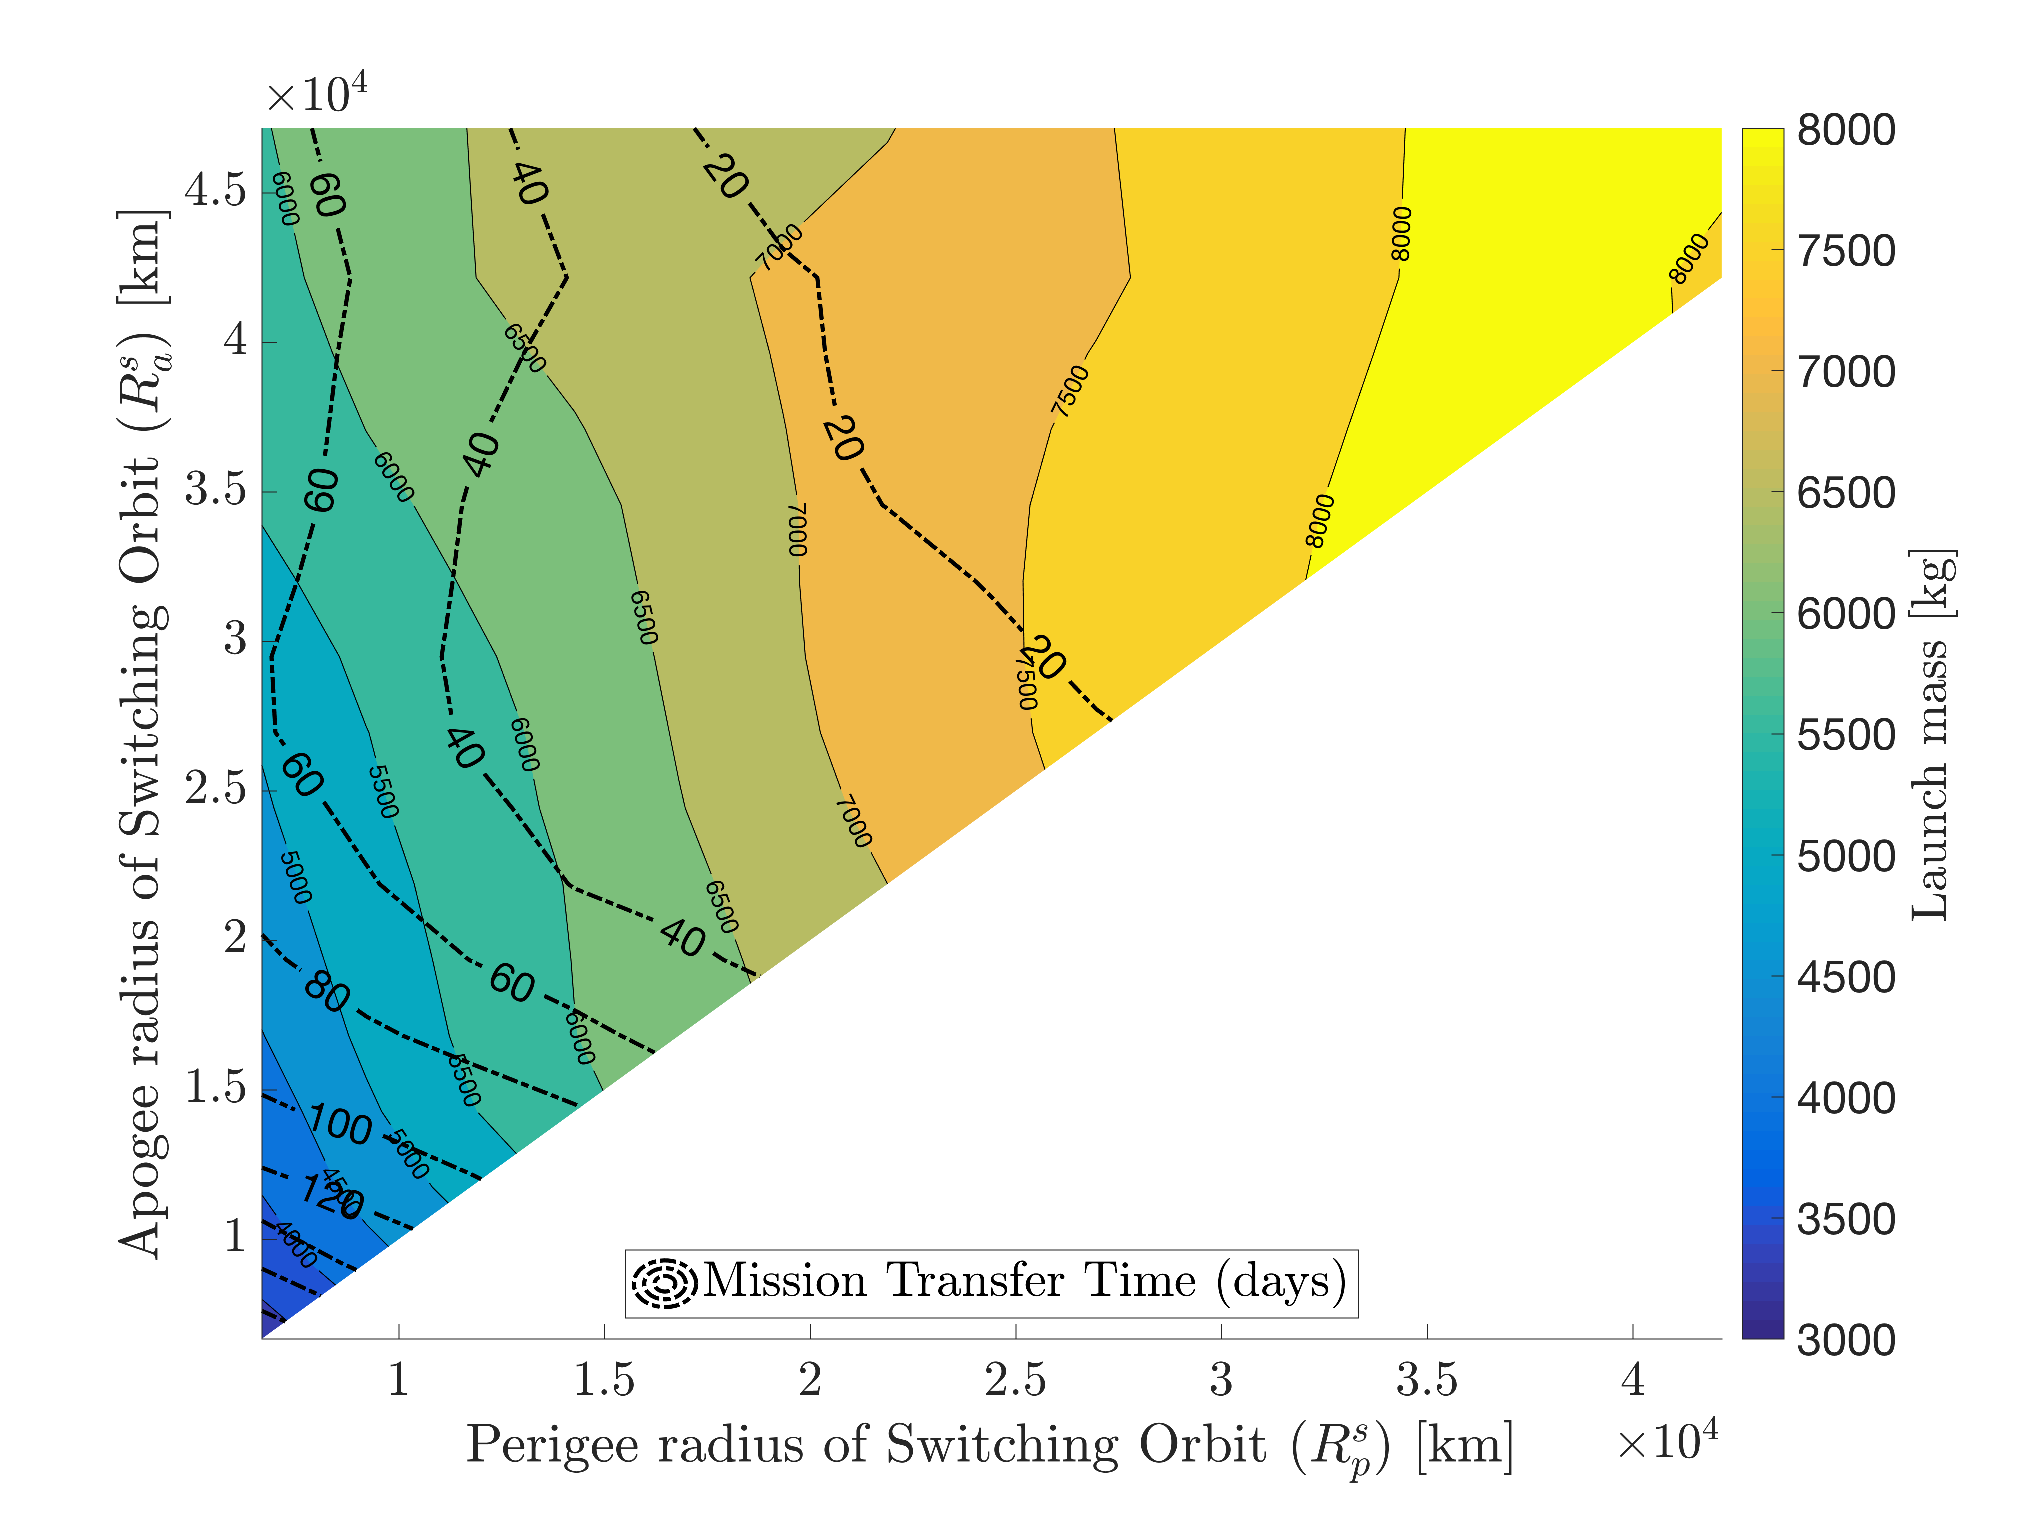
\includegraphics[width=0.5\textwidth]{initialmass_transfer.eps}
\caption{\textbf{Delivered mass in LEO and transfer time to reach GEO}}
\label{fig:mleotimegeoparametric}
\end{figure}
%
\\
The jettisoned CPM, which occurs along a generic switching orbit (Sec.\ref{subsec:chemicalpropulsionsystem}), is outlined in \figurename\ref{fig:cpmmass}. The FCT does not consider the jettisoning phase.
%
\begin{figure}[htp]
\centering
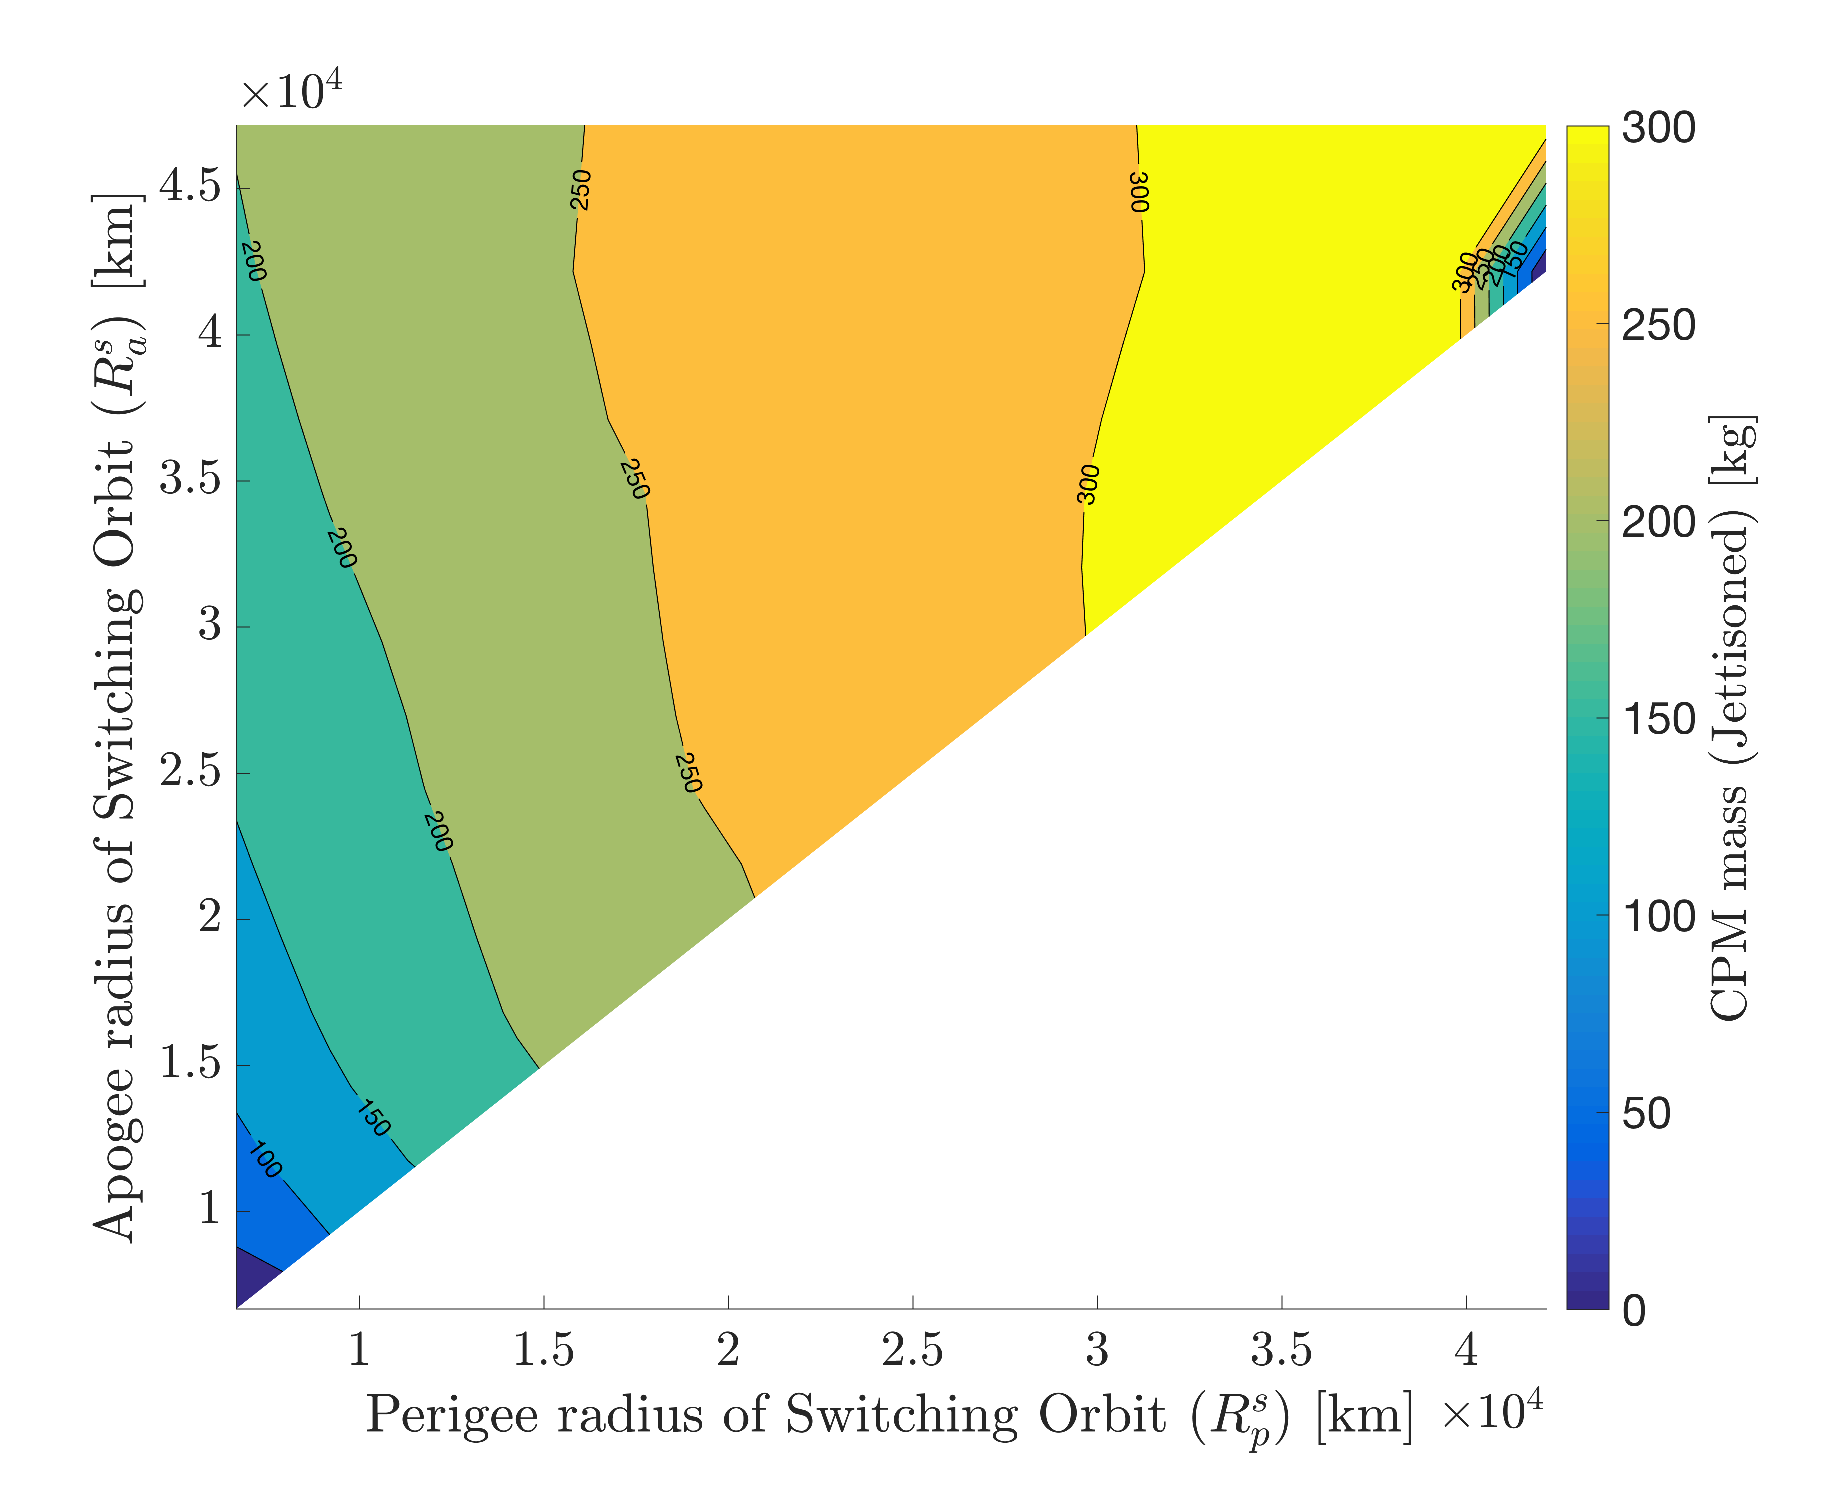
\includegraphics[width=0.5\textwidth]{cpm_jettisoned.eps}
\caption{\textbf{Chemical Propulsion Module CPM mass}}
\label{fig:cpmmass}
\end{figure}
%
It is important to remember and highlight that the most energetic trapped particles (electrons and protons) populate the torus region from a radius of $\sim19000~\si{\kilo\meter}$ to $\sim37000~\si{\kilo\meter}$ mostly~\cite{wertz2011space}. 
At this point, it is easily to attest that the total equivalent fluence of $1~\si{\mega\electronvolt}~e$ in \figurename\ref{fig:equivalentfluencewholemission}, the life degradation factor at the mission EOL in \figurename\ref{fig:ldwholemission}, and the coverglass thicknesses, in \figurename\ref{fig:coverglasswholemission} are consistent to each other and to the physics of the problem.
%
\begin{figure}[htp]
\centering
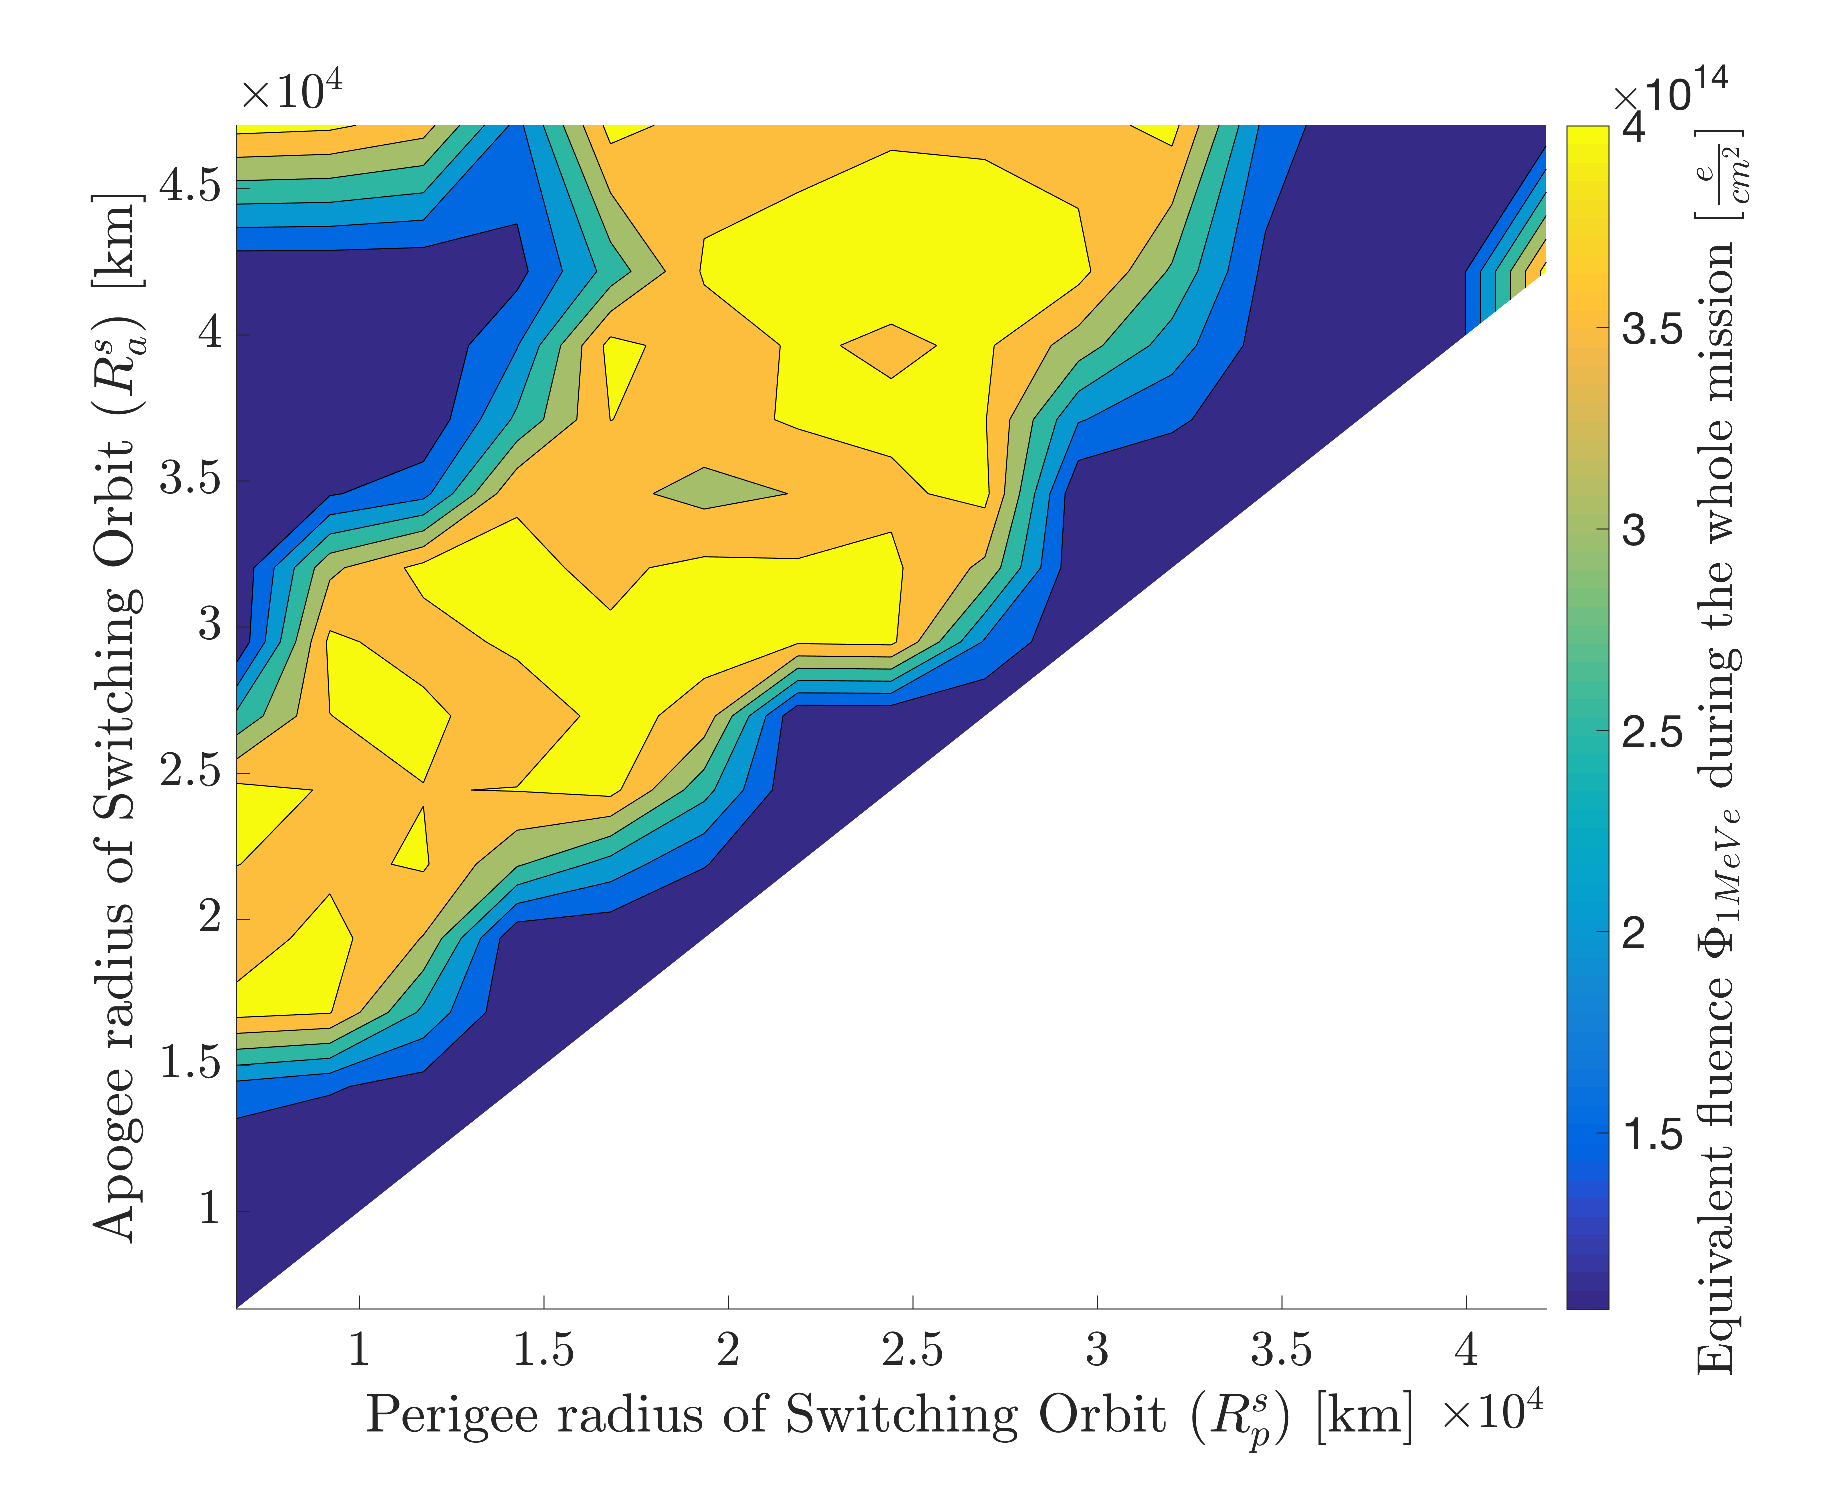
\includegraphics[width=0.5\textwidth]{eqfluence_transfer.eps}
\caption{\textbf{Equivalent fluence of $1~\si{\mega\electronvolt}~e$ during the whole mission lifetime}}
\label{fig:equivalentfluencewholemission}
\end{figure}
%
\begin{figure}[htp]
\centering
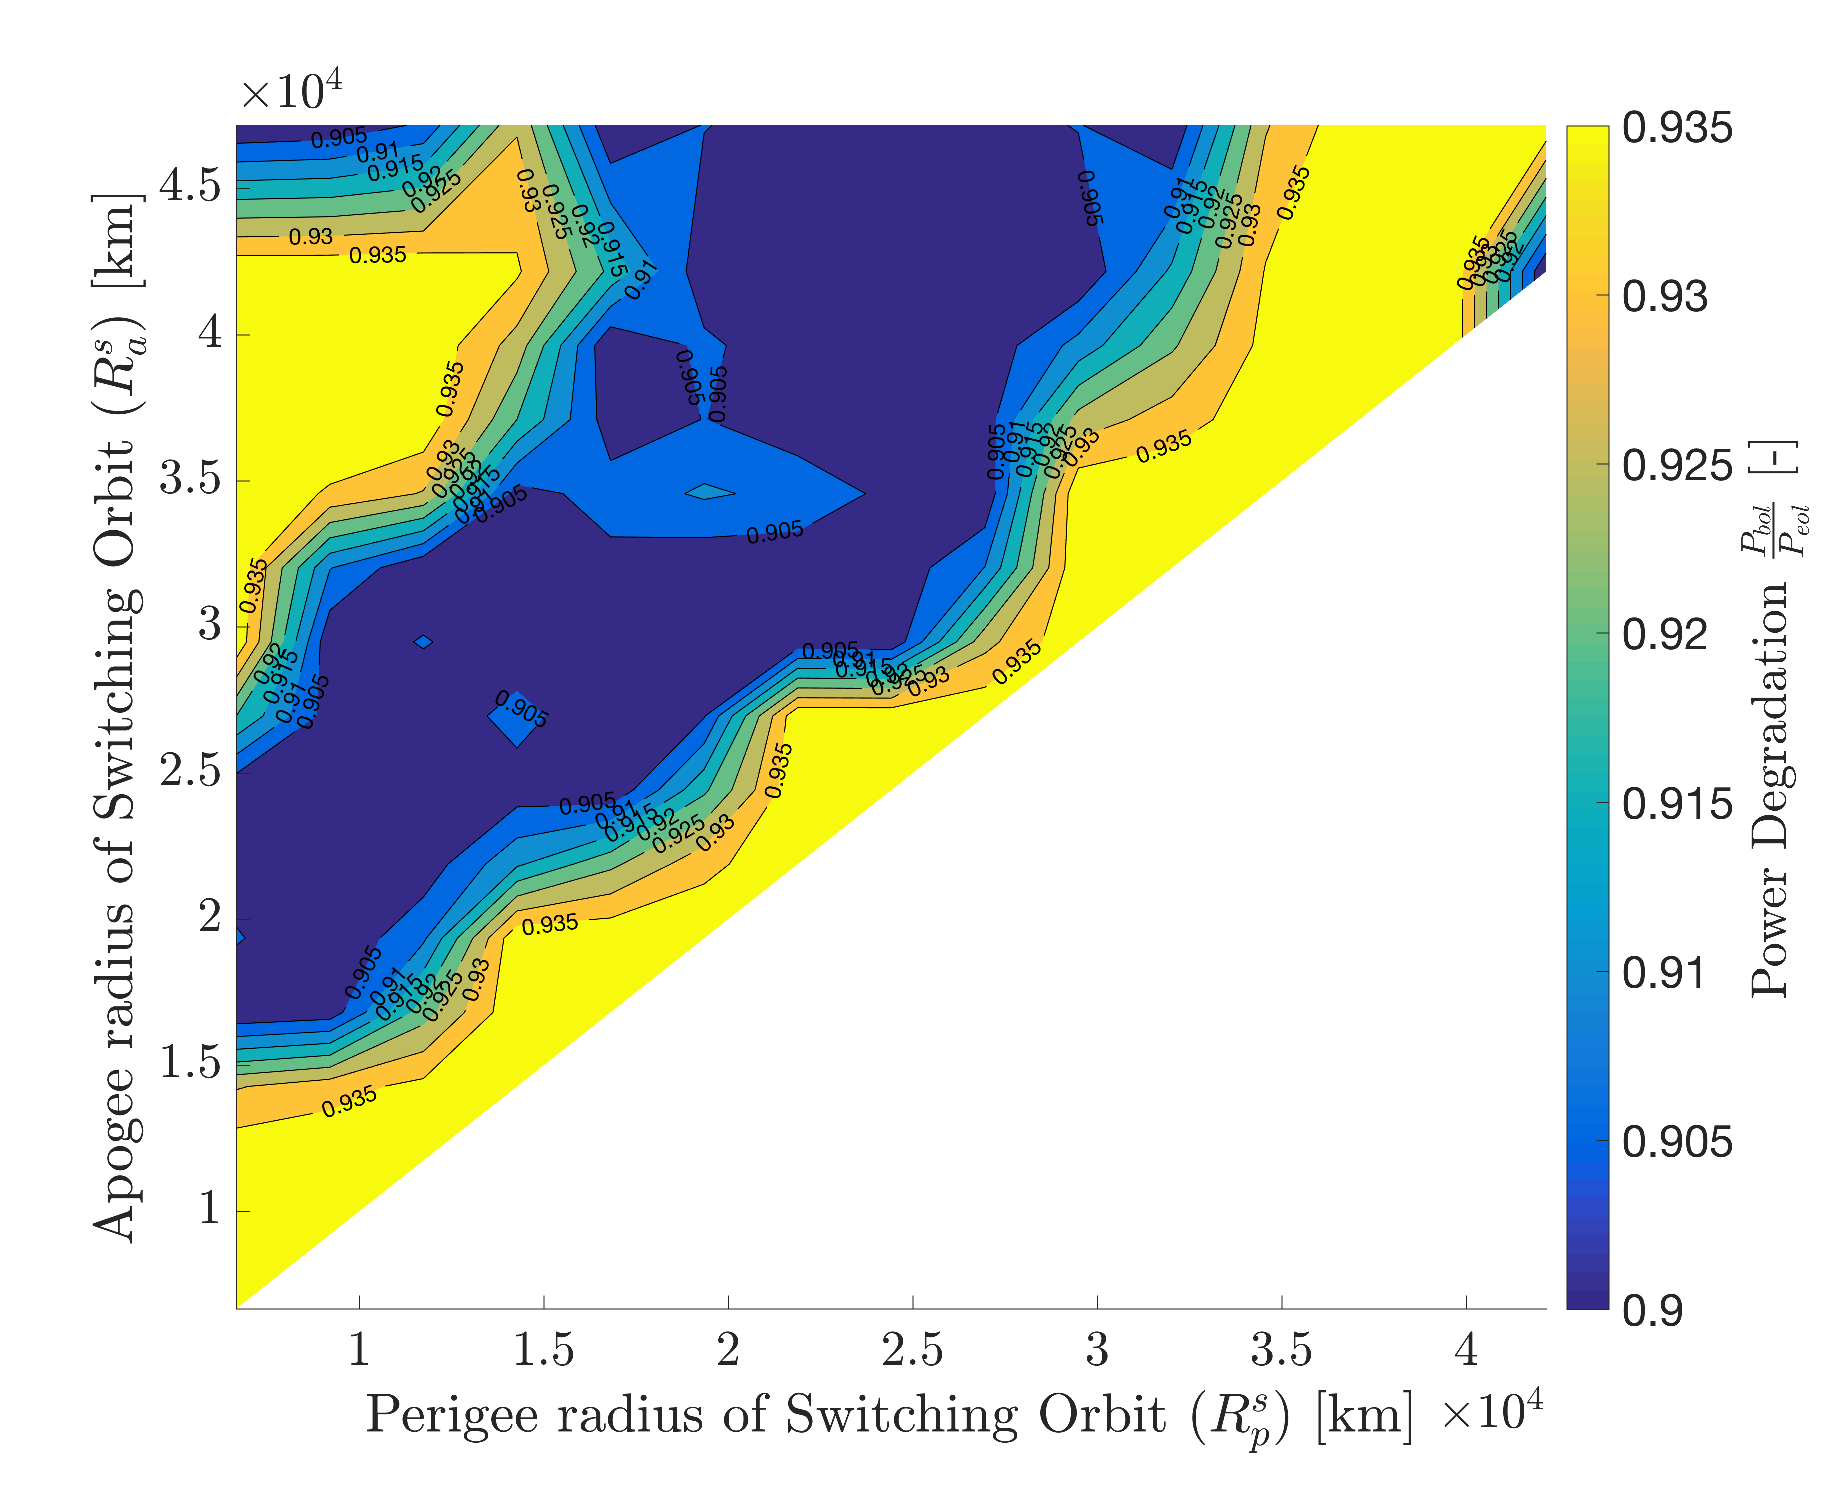
\includegraphics[width=0.5\textwidth]{Ld_transfer.eps}
\caption{\textbf{Available Power from solar array at mission EOL.}}
\label{fig:ldwholemission}
\end{figure}
%
\begin{figure}[htp]
\centering
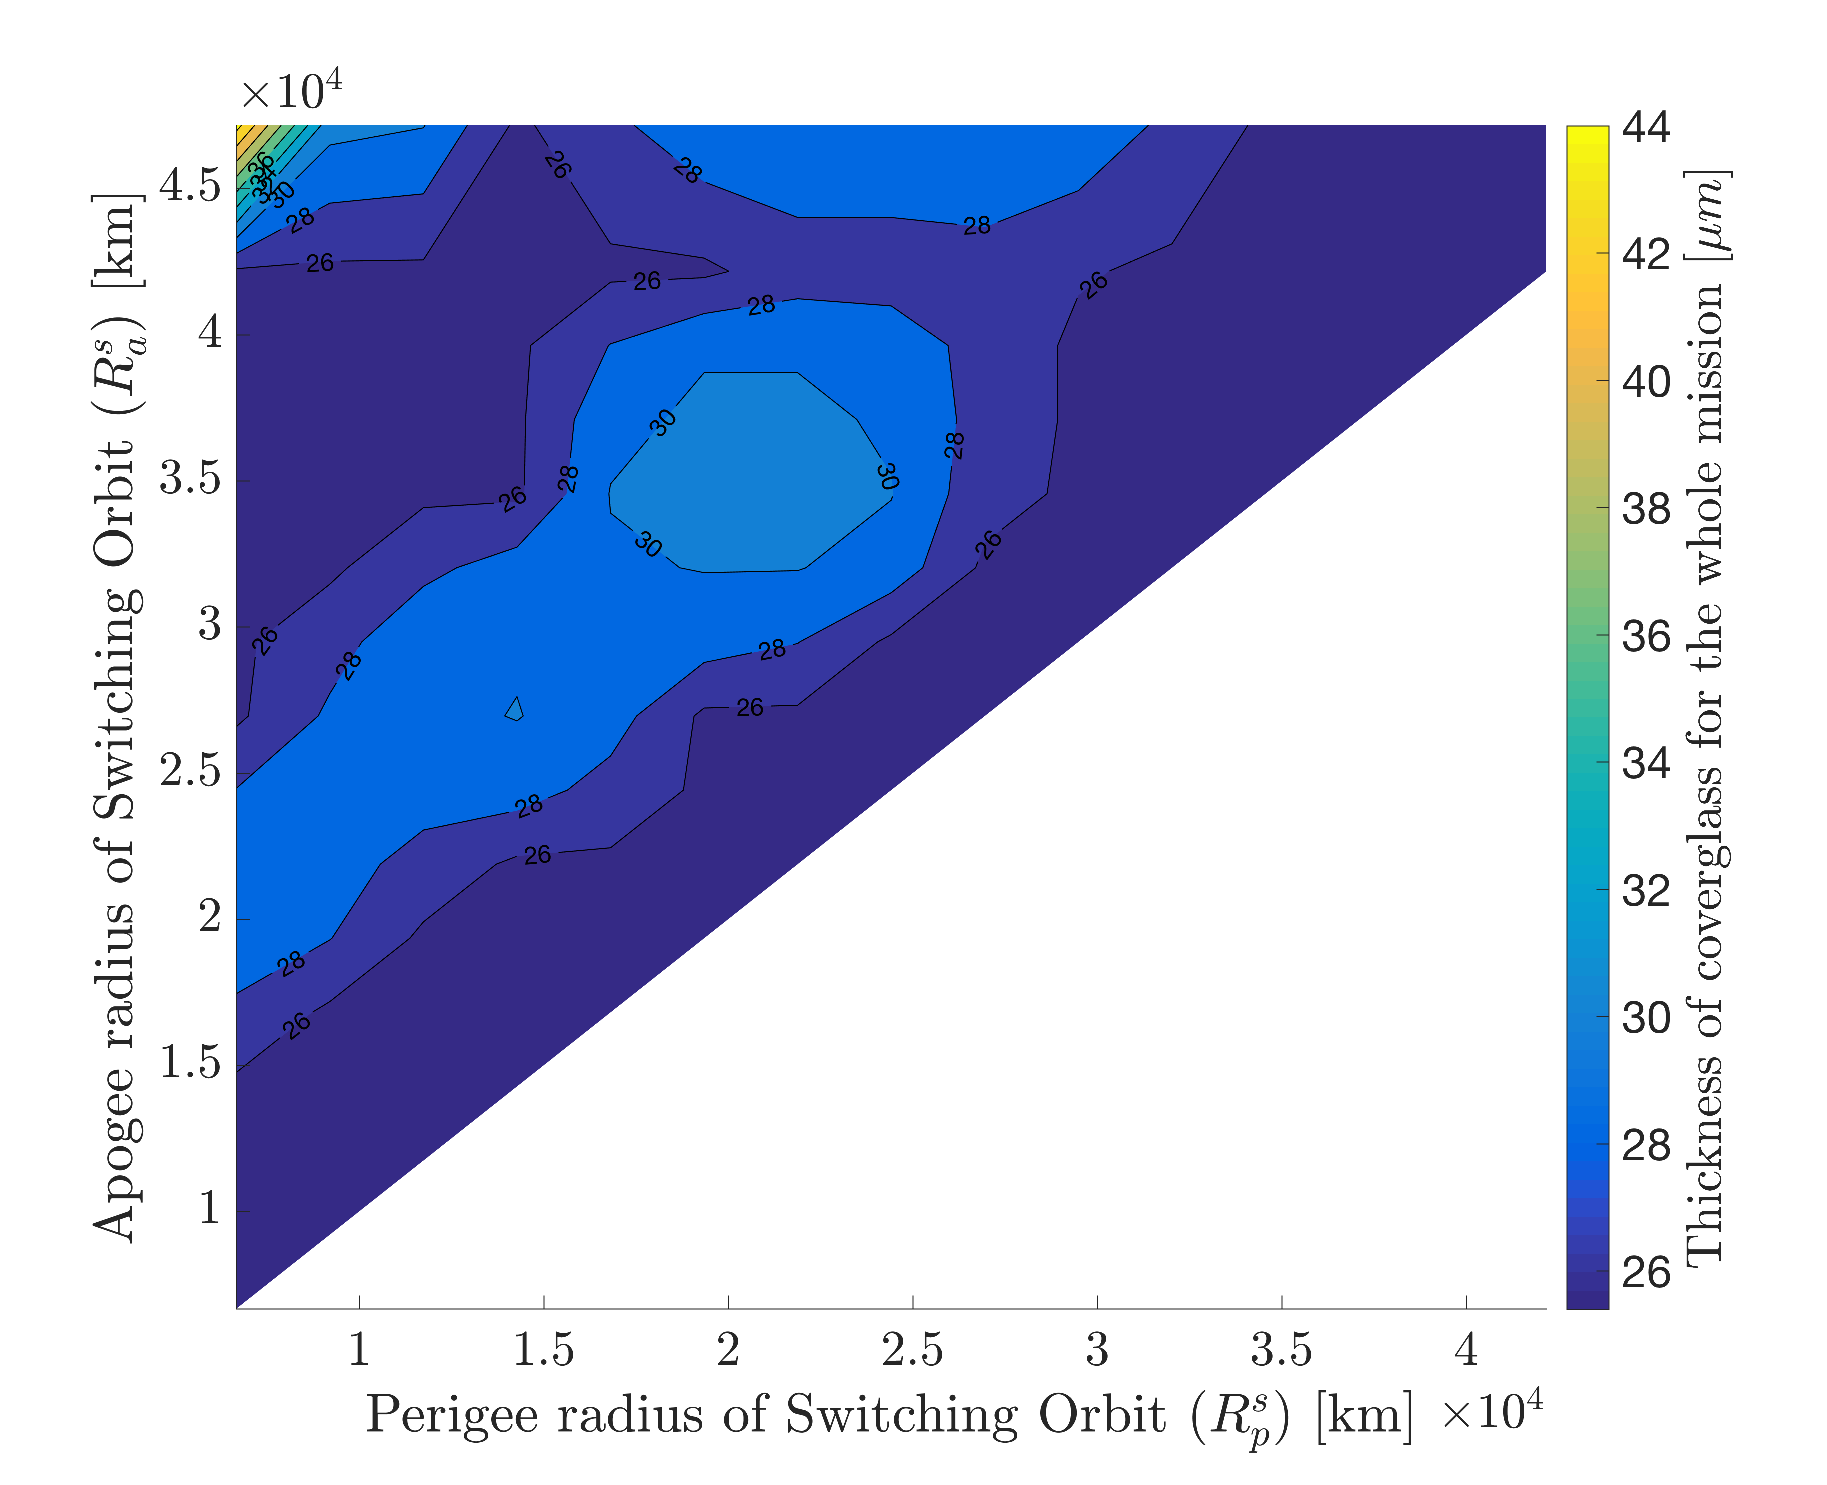
\includegraphics[width=0.5\textwidth]{coverglass_transfer.eps}
\caption{\textbf{Coverglass to shield the solar array during the whole mission}}
\label{fig:coverglasswholemission}
\end{figure}
%
One may affirm that the equivalent fluence connected to the FCT ($R_s^p = R_s^a = R_{\textsc{geo}}$) should have the lowest value among the others since the source of radiation is represented only by the time spent in GEO, see \Eq{eq:radiationcomputation}. 
This statement is not true because the equivalent fluence \eqref{eq:radiationcomputation} is a function of the thickness of coverglass and the solar cell properties in addition to the trajectory-history. 
Consequently, there may be multi-spiral, low-thrust transfer where the equivalent fluence is lower than that of the FCT even though the trapped particles exposure is higher (details in \cite{tesisimo}). The available powers at EOL (\figurename\ref{fig:ldwholemission}) follows the input value ($90\%$) in \tablename\ref{tab:inputscasestudy}.

The mass delivered in GEO is shown in \figurename\ref{fig:deliveredmassingeo}, where one may notice that the more the transfer is accomplished by the bi-impulsive maneuver, the lighter the spacecraft in GEO will be. This is a reasonable characteristic of the HT for a dual stage spacecraft because the closer the switching orbit to GEO, the heavier the CPM jettisoned from the satellite will be.
%
\begin{figure}[htp]
\centering
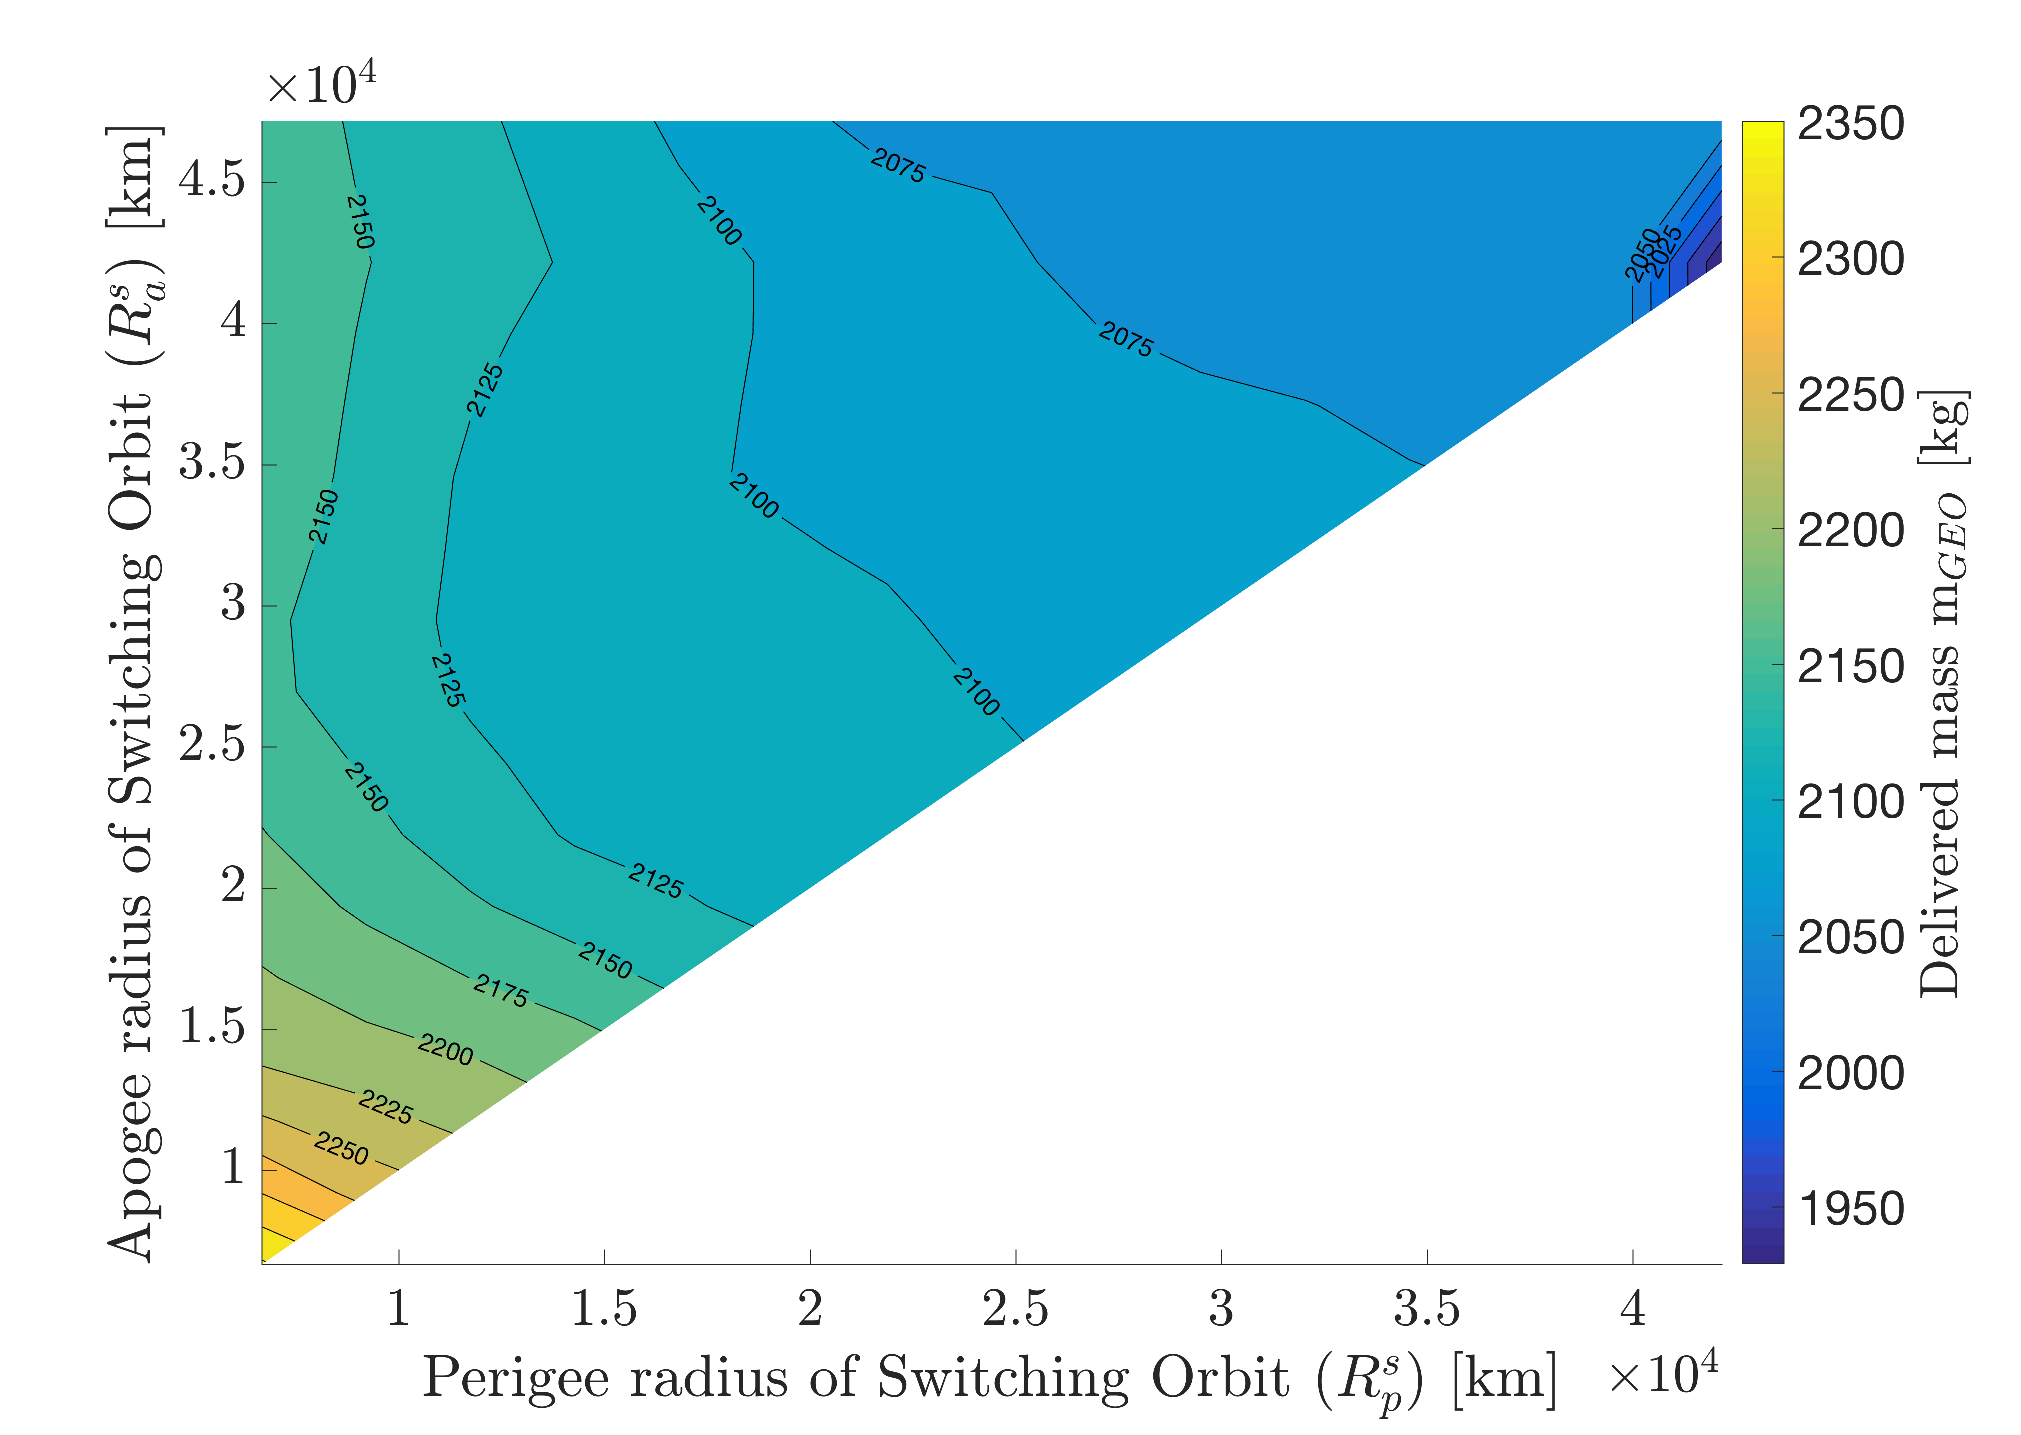
\includegraphics[width=0.5\textwidth]{deliveredmass_geo.eps}
\caption{\textbf{Delivered mass in GEO}}
\label{fig:deliveredmassingeo}
\end{figure}
%
\subsection{Pareto Analysis}
\label{subsec:paretonalaysis}
The figures just described represent the investigation of \emph{Hybrid Transfer} solutions by way of a parametric approach, which eases the concept of \emph{different hybrid transfers means different spacecraft configurations}. 
A key feature to interpret the results lies in understanding which are the solutions to pick among the ones obtained.
Therefore, Pareto optimality chooses the best solutions included in a specified set.
Previously, the results of the orbital dynamics and of the mission cost were functions of the switching orbits mapped through the \emph{Search Grid}.

\figurename\ref{fig:paretomasstime} and \figurename\ref{fig:paretocosttime}, instead, depict the solutions for \emph{Hybrid Transfers} to GEO from different point of views.
The former involves the \emph{time-to-flight vs. launch mass} ($\tau_{\scriptstyle{transfer}}~vs.~m_{\scriptstyle{\textsc{leo}}}$) and the latter works into the \emph{time-to-flight vs. cost of mission} ($\tau_{\scriptstyle{transfer}}~vs.~\$\si\mega$).
Pareto-efficient transfers (the red circles in \figurename\ref{fig:paretomasstime}) broaden the tradespace in GEO mission design.
Moreover, it is shown beyond any doubt that the \emph{Hybrid Transfers} fill the gap between the FCT and the FET by means of a quite smooth trend.
%This can also be verified by analyzing the Table \ref{tab:paretofrontresultstimemass}, where these solutions are listed.
On the other hand, the Pareto-efficient mission costs (the blue triangles in \figurename \ref{fig:paretocosttime}), applied for the \emph{Fiscal Year $2020$}, behave roughly because of the launchers constraint on the mass-at-launch capability.

It is very important to underline and highlight that the Pareto Optimality is used twice because significant inference are drawn, even if they may depend on the implemented preliminary cost-model. 
Pareto-efficient launch masses in LEO (\figurename\ref{fig:paretomasstime}) differ from the Pareto-efficient mission costs (\figurename\ref{fig:paretocosttime}) both quantitatively and qualitatively.
Furthermore, the Pareto-front for mission costs bring to light that the FET does not belong to the set of the best solutions, indeed, there are transfer paths which deliver the payload in GEO in a bit more of half FET time-of-flights for a bit lower mission cost.
%This observation is useful dealing with the development of future satellites because \textbf{maybe}, (and the author emphasizes \emph{maybe}), an all-electric platform to reach \textsc{geo} is not the best solution to achieve the mass-saving and economic revenue purposes simultaneously.
%
\begin{figure}
\centering
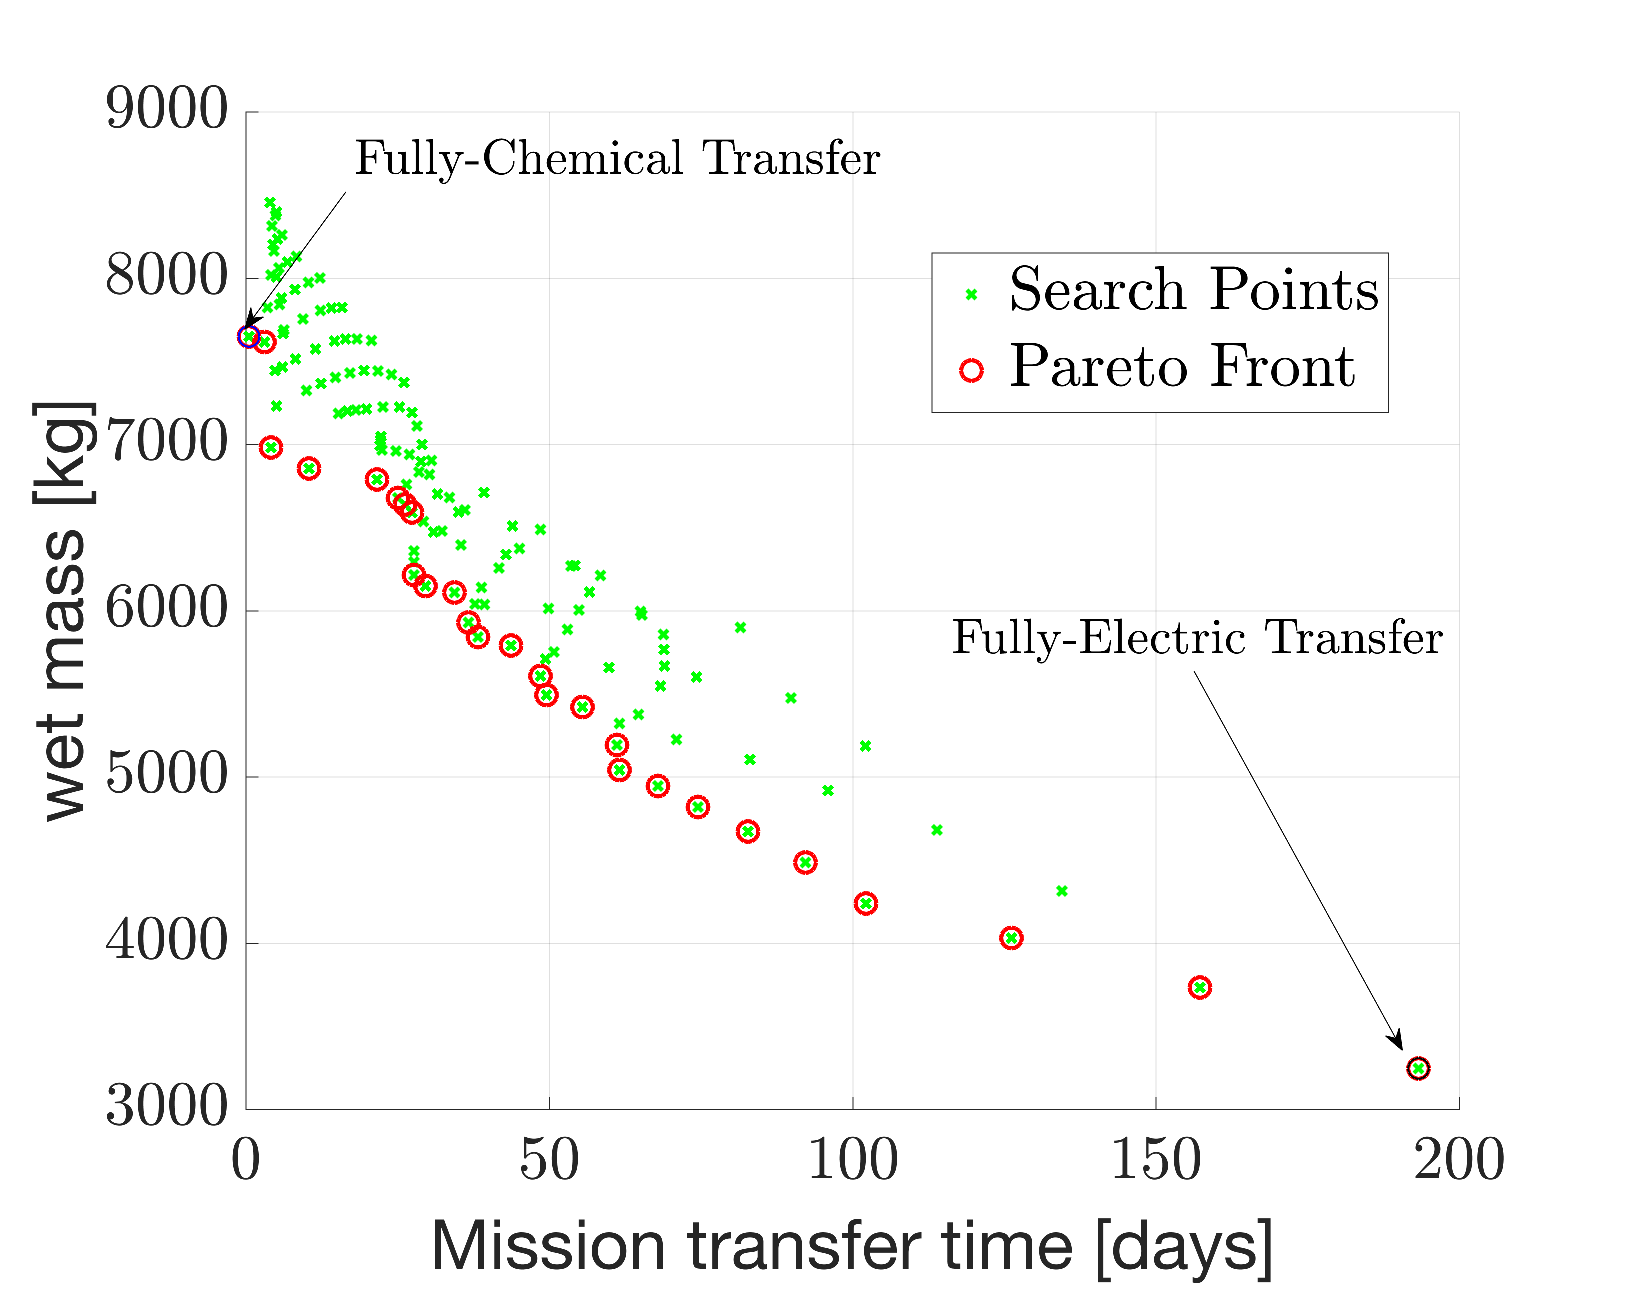
\includegraphics[width=0.5\textwidth]{masstime_pareto.eps}
\caption{\textbf{Pareto front for Launch Mass-vs-Transfer Time}}
\label{fig:paretomasstime}
\end{figure}
%
\begin{figure}
\centering
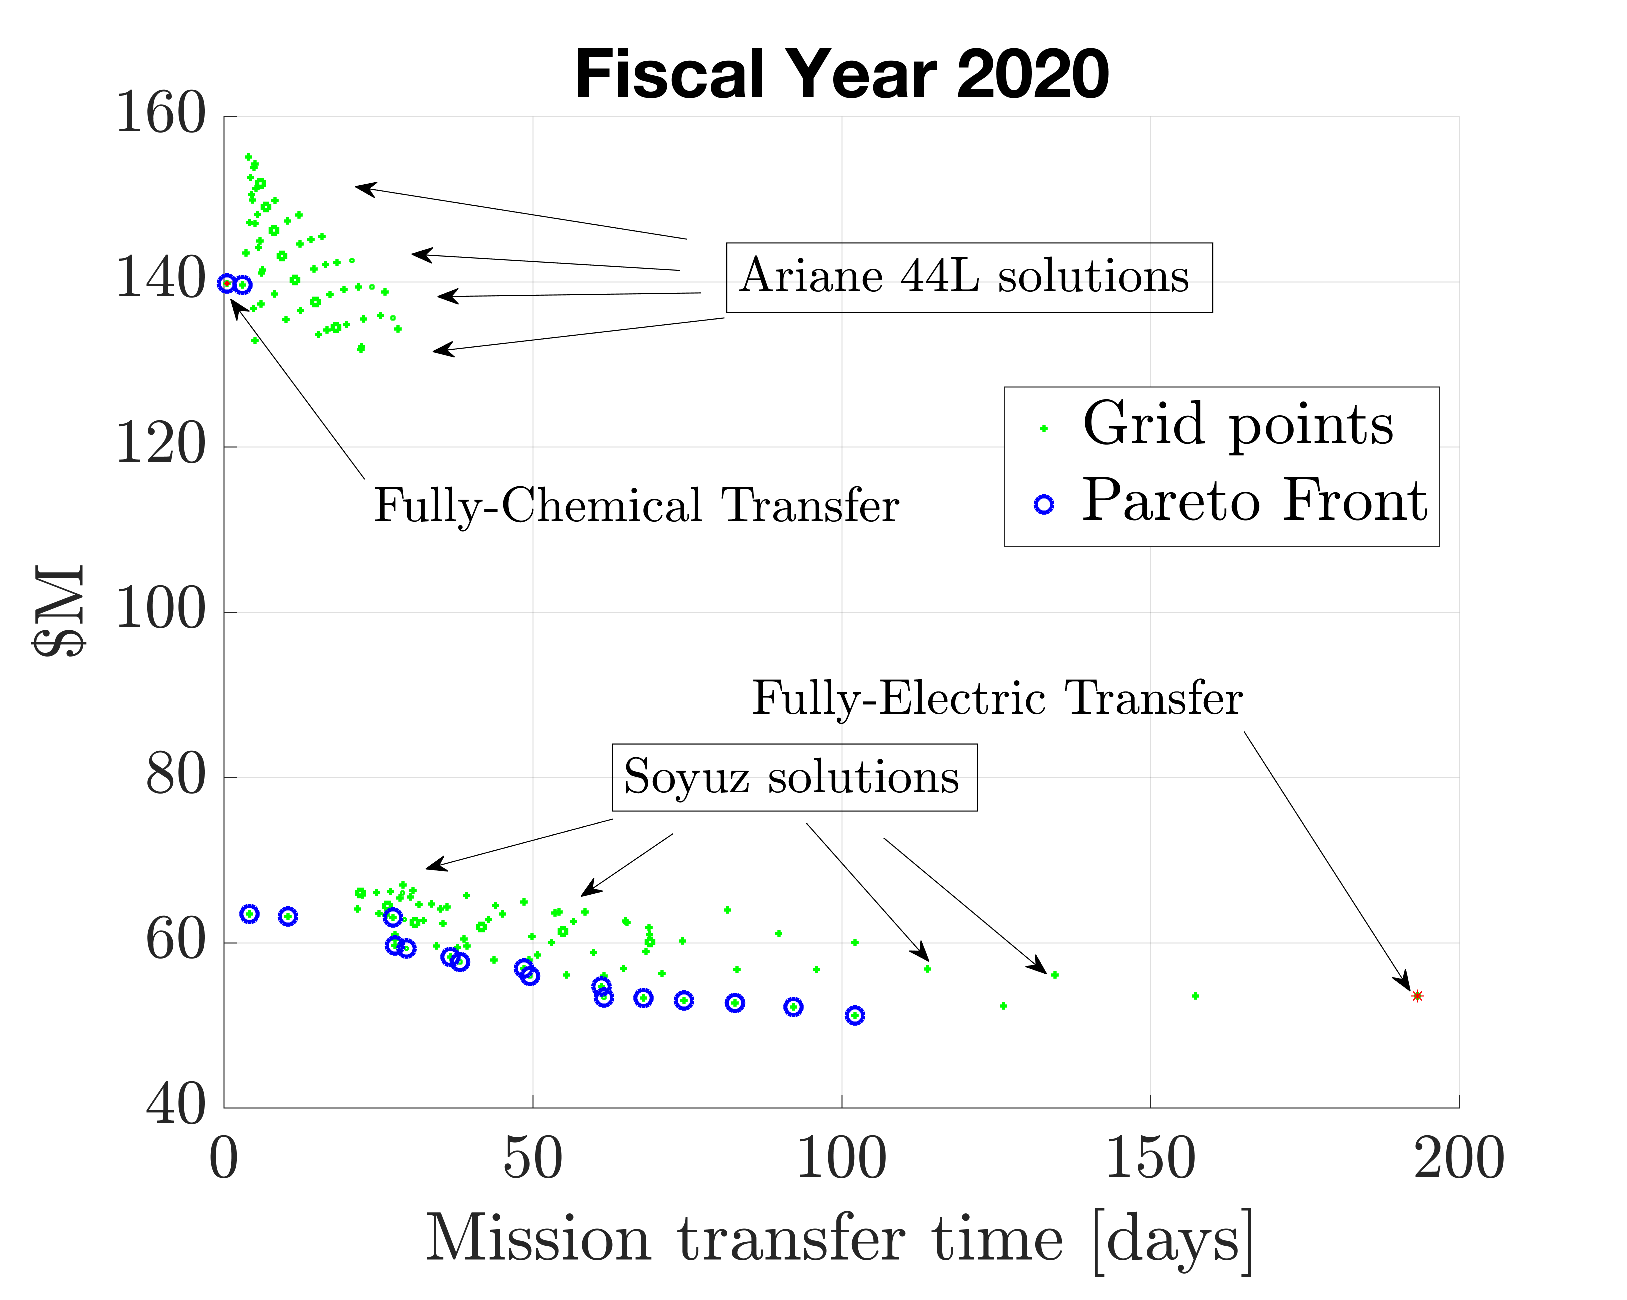
\includegraphics[width=0.5\textwidth]{costtime_pareto.eps}
\caption{\textbf{Pareto front for Cost Mission-vs-Transfer Time}}
\label{fig:paretocosttime}
\end{figure}
%